A Wireless Sensor Network is a collection of a huge number of sensor
nodes that are spread over a wide area and are responsible for
sensing, storing and transmitting information. A typical sensor node
consists of a radio, responsible for transmitting and receiving
information; a battery, which is the main energy source; a
micro-controller, which is a small computer on a chip, responsible for
performing computation and processing; an analog circuit and a sensor
interface.

Research on WSNs has been quite prevalent over the past decade as they
can be easily deployed in harsh environmental conditions, they are
cheap and are easy to maintain. More recently, advancements in
wireless technologies and wireless communication has led to widespread
use of sensors in applications like health, military, security,
agriculture, and wildlife monitoring. With such advancements, research
has also spread into several domains and has led to the development of
several architectures for sensor arrangement
\cite{akyildiz2002wireless}; made deployment of sensors easier; made
them cheaper and made them more scalable than ever. WSN sensor
architectures are commonly implemented in either centralized or
distributed fashion.  In a centralized network, the sink node (which
is usually considered to have unlimited resources in terms of
processing and energy) has complete control of the network and is
responsible for sensor deployment and resource allocation. This means
there is less burden on the sensor nodes and no self-organization
costs are inposed on them. On the other hand, in a distributed
network, sensors govern themselves and are responsible for deployment,
allocation of resources and communication with neighboring sensors to
transmit information to the sink node.

Let us consider an example scenario where a number of cheap, dumb
sensors are spread over an agricultural field in a distributed manner
to monitor agricultural factors like amount of water required for
cultivation, amount of fertilizer required, depth at which a seed must
be sown, etc. A decentralized arrangement for this network has the
following flaws: first, each sensor communicates with its neighboring
sensor(s) to transmit its information and, at the same time, it is
involved in passing information of other sensors' data
\cite{akyildiz2002wireless}. This means that the number of
communications being performed by each sensor in such a setting is
potentially greater than the network's energy budget can afford, as we
know that data transmission consumes more energy than any other sensor
network activity \cite{torres2006energy}. Hence, such an approach will
deplete the sensors' energy in short order, and the expensive process
of retrieval and redeployment must take place. Second, certain sensors
located close to the sink get exhausted quicker in comparison to other
sensors, as most sensors' data needs to pass through one of these
sensors \cite{heinzelman2002application}. Hence, for scenarios like
the one mentioned above and many others like monitoring of buildings,
it is often advisable to opt for a centralized architecture like the
one depicted in Figure \ref{cwsn}, which eliminates the flaws
mentioned above.

\begin{figure}
\begin{center}
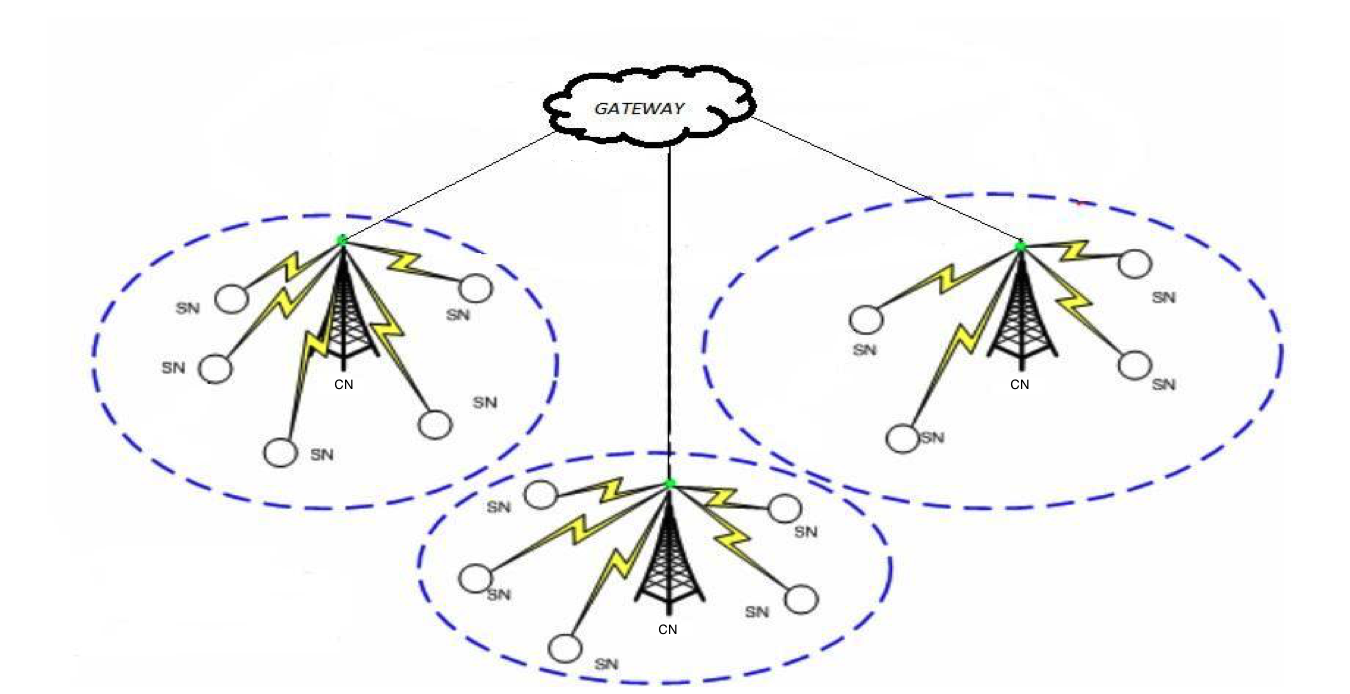
\includegraphics[height = 80mm, width = 150mm, scale = 2]{figs/CWSN}
\caption{A centralized WSN solution to WSNs on an energy budget}
\label{cwsn}
\end{center}
\end{figure}

However, in order to take advantage of the benefits mentioned above,
we will have to deal with several problems associated with
WSNs. Probably the most important of such problems is to improve the
energy-efficiency of the sensors within the WSN. This is because the
sensors ordinarily have small, low-capacity batteries as their only
energy source. Once a battery is drained it can be very expensive to
replace it, and more importantly, we will lose the ability of the
network to give us an accurate measure of the sensing environment
during the period when the sensor is offline. Hence, it is crucial
that we prolong the lifetime of sensors by improving the energy
efficiency of a sensor network deployment scheme. Over the years,
several approaches have been proposed to address this problem.

Another problem lies in the fact that not all the sensors at every
moment of time provide the best information. Most of the time, sensors
send redundant information, which is non-informative in terms of
entropy. Many approaches like data fusion, data aggregation,
clustering etc. have been proposed to reduce redundant data
\cite{abbasi2007survey} \cite{rajagopalan2006data}. Also, several
approaches have been proposed in order to maximize the amount of
information gathered from a system \cite{ji2014data}. This problem has
also been proven as NP-Hard \cite{chou2009energy}.

In this paper, we propose an approach that makes use of Information
Entropy to determine the theoretical upper bound on the VoI available
in a network and to increase the amount of information gathered from
the network. We achieve this by identifying the most informative
sensors consistently and query/ping them more often on comparison to
others, thereby increasing the overall information gathered from the
system.

In order to show energy-efficiency, our approach varies the rate of
sampling to prove that it gathers more information from the sensors
even at low sampling rates, instead of transmitting information to the
central node whenever a change is seen -- which eventually leads to
making excessive, unnecessary transmissions and depleting the sensors'
energy more quickly. The simulation results shown below are concrete
proof that our approach (in comparison with two state-of-the-art
models) gathers more information at every ping rate taken into
consideration. These results are further evidence for the fact that
our model gathers more information per ping and is energy-efficient in
comparison.